% =============================================================================
% 3. RESOLUCION DE TAREAS  (40 %)
% Espacio: ~1,8 paginas.
% El enunciado pide: traza breve con resultados intermedios + evolucion del tiempo con la talla.
% =============================================================================
\section{Resolución de tareas}
\label{sec:tareas}

\pendiente{presentación breve de las tareas resueltas (Tabla~\ref{tab:tareas}) y del método
  usado en cada tier.}

% ---------------------------------------------------------------- Estado de las tareas
% Una casilla por tarea: \est{ok} resuelta y comprobada (solo estas suman puntos),
% \est{aprox} resuelta sin certificar el optimo, \est{pend} pendiente.
% \tier{n} al principio de cada fila indica a que tier suman las casillas "ok".
% Estado a 12/11: GGH Tier0 comprobadas con la solucion del fichero; resto de GGH con
% LLL + Babai (Tier02T03 no es la optima); GGH modulares (m), LWE y Ring-LWE sin hacer.
\begin{table}[H]
\centering\small
\setlength{\tabcolsep}{5pt}
\begin{tabular}{@{}l c ccccccc@{}}
  \toprule
  Criptosistema & Tier & T01 & T02 & T03 & T04 & T05 & T06 & T07 \\
  \midrule
  \multirow{4}{*}{GGH}
    & 0 & \tier{0}\est{ok} & \est{ok} & \est{ok} & \est{ok} & \est{ok} & & \\
    & 1 & \tier{1}\est{aprox} & \est{aprox} & \est{aprox} & \est{aprox} & \est{aprox} & \est{aprox} & \est{aprox} \\
    & 2 & \tier{2}\est{aprox} & \est{aprox} & \est{pend} & \est{aprox} & \est{aprox} & & \\
    & 3 & \tier{3}\est{pend}$^m$ & \est{pend}$^m$ & \est{aprox} & \est{aprox} & \est{pend}$^m$ & & \\
  \midrule
  \multirow{4}{*}{LWE}
    & 0 & \tier{0}\est{pend} & \est{pend} & \est{pend} & \est{pend} & \est{pend} & & \\
    & 1 & \tier{1}\est{pend} & \est{pend} & \est{pend} & \est{pend} & \est{pend} & & \\
    & 2 & \tier{2}\est{pend} & \est{pend} & \est{pend} & \est{pend} & \est{pend} & & \\
    & 3 & \tier{3}\est{pend} & \est{pend} & \est{pend} & \est{pend} & \est{pend} & & \\
  \midrule
  Ring-LWE
    & 3 & \tier{3}\est{pend} & \est{pend} & \est{pend} & & & & \\
  \bottomrule
\end{tabular}

\vspace{2pt}{\footnotesize Puntuación (solo tareas comprobadas): \puntuacion}
\caption{Estado de las tareas. $\checkmark$: resuelta y comprobada; $\approx$: resuelta sin
  certificar que sea la óptima; --: pendiente; $^m$: celosía con reducción módulo $n$.}
\label{tab:tareas}
\end{table}

% ---------------------------------------------------------------- Resultados
% Solo tareas representativas (no caben todas): al menos una por algoritmo.
\begin{table}[H]
\centering\small
\begin{tabularx}{\linewidth}{@{}l c l Y r@{}}
  \toprule
  Tarea & Talla & Método & Resultado & Tiempo (s) \\
  \midrule
  \falta{Tier0T01\_Latt}  & \falta{2}  & \falta{LLL + Babai}    & \falta{} & \falta{} \\
  \falta{Tier3T01\_LWE}   & \falta{}   & \falta{ataque primal}  & \falta{} & \falta{} \\
  \falta{Tier3\_T01\_LWE} & \falta{16} & \falta{sistema lineal} & \falta{} & \falta{} \\
  \bottomrule
\end{tabularx}
\caption{Resultados de tareas representativas (una por método).}
\label{tab:resultados}
\end{table}

% ---------------------------------------------------------------- Trazas
% Una traza corta por algoritmo con los resultados intermedios de una ejecucion real.
% Copiar la salida del programa (recortada) dentro de cada una.
\begin{traza}{Tier0T01\_Latt, LLL + Babai.}
\falta{base pública}\\
\falta{base tras LLL}\\
\falta{coordenadas antes y después de redondear}\\
\falta{punto obtenido}
\end{traza}

\begin{traza}{Tier3T01\_LWE, ataque primal.}
\falta{dimensión de la celosía}\\
\falta{fila de la base reducida que contiene el error}\\
\falta{secreto $s$ y comprobación $b - As$}
\end{traza}

\begin{traza}{Tier3\_T01\_LWE, Ring-LWE.}
\falta{$b$ centrado; $s$ obtenido; error $e = b - a\,s$}\\
\falta{$d = c_2 - s\,c_1$ centrado y palabra de bits}
\end{traza}

% ---------------------------------------------------------------- Tiempo frente a talla
\begin{figure}[H]
  \centering
  % Grafica de tiempo frente a talla (el enunciado la pide).
% Lee un CSV por metodo en datos/, que debe generar scripts/bench.py:
%
%   datos/tiempos_ggh_lll_babai.csv        talla,segundos
%                                          2,0.0003
%                                          15,0.016
%
% Cada linea \serie{...} de abajo es un metodo: si su CSV no existe, no se dibuja.
% Mientras no exista el de GGH (LLL + Babai), se muestra un aviso en su lugar.

% \serie{metodo}{estilo de linea}{marca}{leyenda}
\newcommand{\serie}[4]{%
  \IfFileExists{datos/tiempos_#1.csv}{%
    \addplot[black,#2,mark=#3,mark options={solid}]
      table[x=talla,y=segundos,col sep=comma]{datos/tiempos_#1.csv};
    \addlegendentry{#4}}{}}

\IfFileExists{datos/tiempos_ggh_lll_babai.csv}{%
  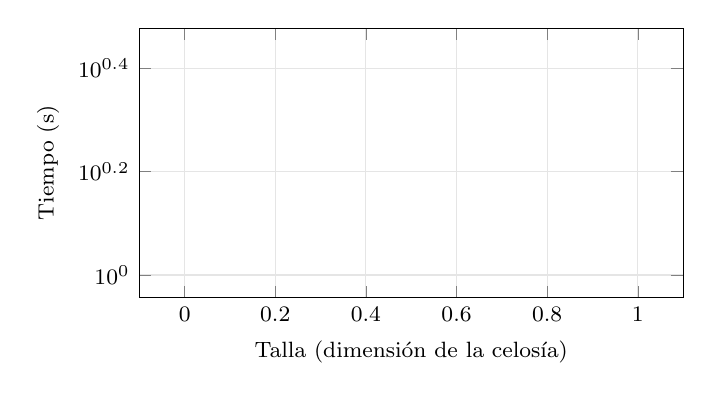
\begin{tikzpicture}
    \begin{semilogyaxis}[
        width=0.7\linewidth,height=5cm,
        xlabel={Talla (dimensión de la celosía)},ylabel={Tiempo (s)},
        font=\footnotesize,
        grid=major,grid style={gray!20},
        legend pos=outer north east,legend cell align=left,
        legend style={draw=none,font=\scriptsize},
        every axis plot/.append style={line width=0.6pt,mark size=1.6pt}]
      \serie{ggh_lll_babai}{solid}{*}{GGH: LLL + Babai}
      \serie{ggh_enumeracion}{solid}{square}{GGH: enumeración}
      \serie{ggh_fuerza_bruta}{solid}{triangle}{GGH: fuerza bruta}
      \serie{lwe_fuerza_bruta}{dashed}{triangle*}{LWE: fuerza bruta}
      \serie{lwe_primal}{dashed}{*}{LWE: ataque primal}
      \serie{ring}{dotted}{diamond*}{Ring-LWE}
    \end{semilogyaxis}
  \end{tikzpicture}%
}{%
  \pendiente{gráfica tiempo frente a talla. Aparece sola cuando existan los CSV de
    \texttt{report/datos/} (formato en \texttt{figuras/tiempos.tex}), generados por
    \texttt{scripts/bench.py}.}%
}

  \caption{Tiempo de resolución frente a la talla del problema (escala logarítmica).}
  \label{fig:tiempos}
\end{figure}

\pendiente{comentario de la gráfica: qué método crece más rápido y a partir de qué talla deja de
  ser viable.}
